%! TEX root = ../barycenter.tex
\YYCleverefInput{/var/tmp/latex/barycenter.sed}
\section{Barycenter in Wasserstein space}

Recall that we only need Polish space to define Wasserstein metric, so we can write $\mathcal{W}_p(\mathcal{W}_p(E))$
by \cref{thm:topology_Wasserstein} if $E$ is a Polish space.
We always assume that $p \in [1, \infty)$.
And we slightly generalize the definition for barycenter $\mu \in \mathcal{W}_p(E)$
of $\mathbb{P} \in \mathcal{W}_p(\mathcal{W}_p(E))$,
\[
	\text{barycenter } \mu \in \arg \min_{\nu} \int_{\mathcal{W}_p(E)} W_p(\nu, \eta)^p \diff \mathbb{P} (\eta).
\]
The difference here is that squared distance function is replaced by power $p$ of distance function.
Most discussion could be generalized in this way as well.

\subsection{Convention, or abuse of language}

\label{subsection:convention}
Here we make use of \cref{example:delta_measure_Wasserstein_distance}.
Following will be recalled when necessary.

\begin{itemize}
	\item $(E,d)$ a Polish space, $p \in [1, \infty)$.
	\item Points $x,y,z \in E$; $\mu, \nu, \eta \in \mathcal{W}_p(E)$; $\mathbb{P} \in \mathcal{W}_p(\mathcal{W}_p(E))$.
	\item $X$, random variables with values in $(E, d)$.
	\item $W_p$, Wasserstein metric of $\mathcal{W}_p(E)$ and $\mathcal{W}_p(\mathcal{W}_p(E))$.
	\item $W_p(\mu, E):= \inf_{x \in E}W_p(\delta_x, \mu)$,
	      as $x \mapsto \delta_x$ is an isometric embedding.

	      If barycenter $z$ of $\mu$ exists, then $W_p(\mu, \delta_z)=W_p(\mu, E)$.
	\item $W_p(\mathbb{P}, \mathcal{W}_p(E)) := \inf_{\nu \in \mathcal{W}_p(E)} W_p(\delta_\nu, \mathbb{P})$, by isometric embedding again.

	      If barycenter $\mu$ of $\mathbb{P}$ exists, then $W_p(\mathbb{P}, \delta_\mu)=W_p(\mathbb{P}, \mathcal{W}_p(E))$.
	\item $\mu_n \rightharpoonup \mu$ stands for weakly convergence of measures.

\end{itemize}

\subsection{An example on the sphere}

As we saw in previous chapter,
\cref{prop:barycenter_midpoint} states that one can compute barycenter as midpoint in a length space.
Following theorem (\cite[Corollary 7.22]{villani2008optimal}) states that Wasserstein space over a proper and geodesic space is geodesic.

\begin{thm}[Displacement interpolation as geodesics]
	\label{thm:geodesic_Wasserstein_space}
	Let \( ( E , d ) \) be a complete separable, locally compact length space (thus a proper and geodesic space).
	Let \( p > 1 \) and let \( \mathcal{W}_p(E) \) be the space of probability measures
	on \( E \) with finite moment of order \( p \),
	metricized by the Wasserstein distance \( W _ { p } \).
	Then, given any two \( \mu _ { 0 }\), \( \mu _ { 1 } \in \mathcal{W}_p(E) \),
	and a continuous curve \( \left( \mu _ { t } \right) _ { 0 \leq t \leq 1 } \),
	valued in \( \mathcal{W}_p(E) \),
	the following properties are equivalent:
	\begin{enumerate}
		\item \( \mu _ { t } \) is the law of \(\gamma _ { t } \) where \( \gamma \) is a random (minimizing, constant speed)
		      geodesic such that \( \left( \gamma _ { 0 } , \gamma _ { 1 } \right) \) is an optimal coupling;
		\item \( \left( \mu _ { t } \right) _ { 0 \leq t \leq 1 } \) is a geodesic curve in the space \( \mathcal{W}_p(E) \).
	\end{enumerate}
	Moreover, if \( \mu _ { 0 } \) and \( \mu _ { 1 } \) are given, there exists at least one such curve.
\end{thm}

\begin{wrapfigure}{r}{3cm}
	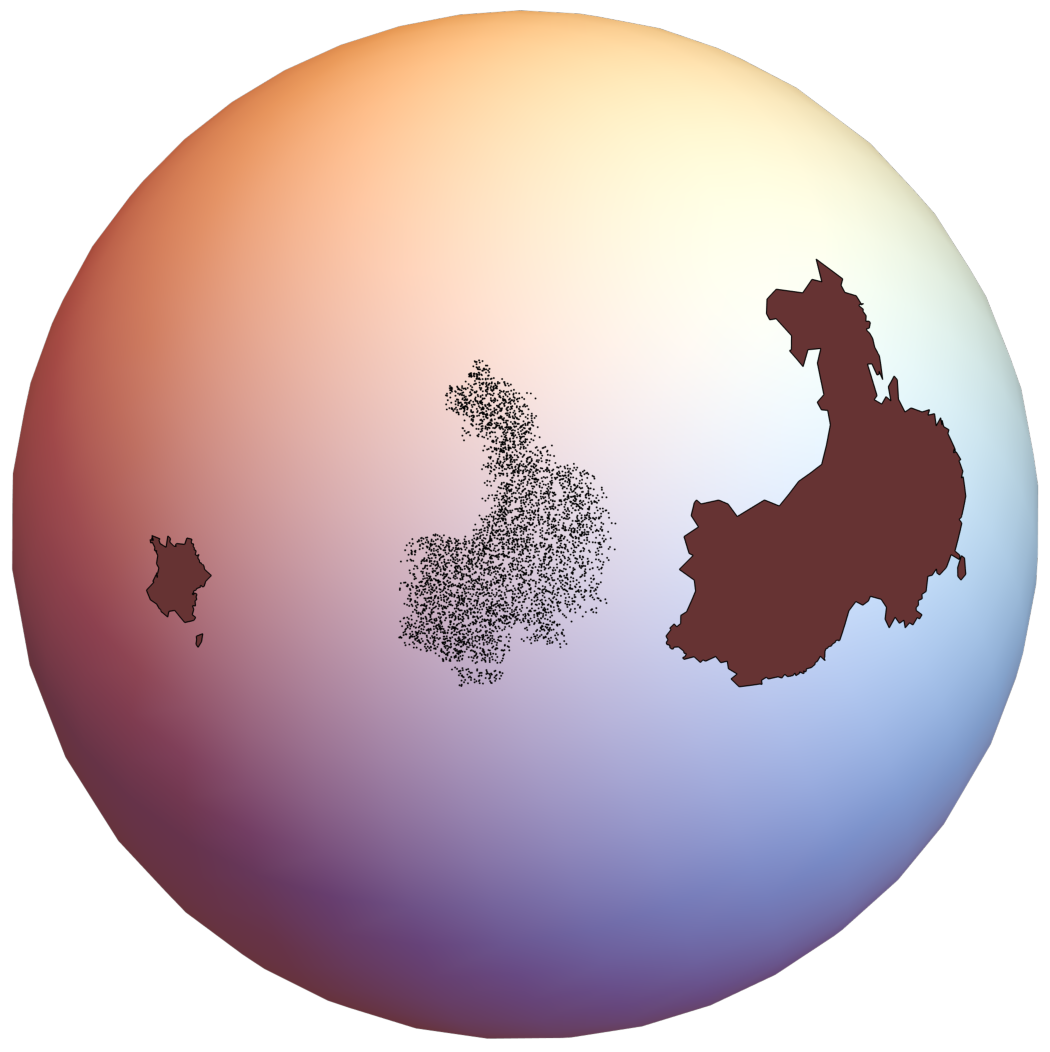
\includegraphics[width=\linewidth]{Chapters/OPT_sphere.pdf}
\end{wrapfigure}

In the right-hand side picture,
the author simulates the unique barycenter between the (mainland) country shapes of France and China.

\begin{example}[Barycenter between France and China]
	\label{example:barycenter_sphere}
	In this setting, $(E, d)$ is the Riemannian manifold of earth sphere.
	In the Wasserstein space $\mathcal{W}_2(E)$, consider two uniform measures $\mu$ and $\nu$,
	with supports on the maps of France and China respectively.
	The aim is to simulate the (unique) barycenter $\eta$ of $\frac{1}{2}\delta_\mu + \frac{1}{2}\delta_\nu$.
	With the help of \cref{thm:geodesic_Wasserstein_space}, we proceed as following.
	We simulate 5000 points for measures $\mu$ and $\nu$.
	Then we compute an optimal matching between those points,
	which costs more than 5 hours in the author's laptop.
	Given these 5000 pairs of points,
	we draw their (unique) barycenters on the sphere and that is a simulation of desired barycenter measure $\eta \in \mathcal{W}_2(E)$.
\end{example}

The source code is shared as a \href{https://www.wolframcloud.com/obj/jingmatrix/Published/OPT_sphere_country.nb}{Wolfram Notebook}.

\section{Existence and consistency}

Results in this section is fully borrowed from \cite{le2017existence}.
We present them in a more geometrical style without the purpose of claiming originality.

Wasserstein space is not locally compact unless the base space is compact (\cite[Remark 7.1.9]{Ambrosio2005}).
But weakly convergence behaves well with Wasserstein metric, and we can get weakly compactness with less cost.
Properness of base space gives ``properness'' of Wasserstein space for \underline{weakly convergence topology}.

\begin{prop}
	\label{prop:proper_weakly_convergence_topology}
	For a proper space $(E,d)$,
	every bounded set in $\mathcal{W}_p(E)$ is tight and thus
	sequentially	pre-compact in weakly convergence topology.
\end{prop}

\begin{proof}
	Closed ball $B(x,r)$ is compact in $E$.
	By Markov inequality,
	\[
		\mu(E - B(x,r)) = \int_{E - B(x,r)} \diff \mu \leq
		\int_{E} \frac{d(x, y)^p}{r^p} \diff \mu(y) \leq  \frac{W_p(\mu, \delta_x)^p}{r^p},
	\]
	and we conclude by the assumption that $W_p( \mu, \delta_x)$ is bounded.
\end{proof}

By abuse of language, we drop $\delta$ symbol in following discussion when there is no ambiguity.
This convention is indicated in \cref{subsection:convention}.
\begin{thm}[Consistency of barycenter in Wasserstein space]
	\label{thm:consistency_barycenter_Wasserstein}
	Let $(E,d)$ be a proper space and $\mathbb{P}_n$  be a sequence in $\mathcal{W}_p(\mathcal{W}_p(E))$
	with barycenter $\mu_n \in \mathcal{W}_p(E)$ and $\mathbb{P}_n \rightarrow \mathbb{P}$ with respect to Wasserstein metric.

	Then $\mu_n$ is tight and any weakly convergence limit $\mu$ of $\mu_n$ will be a barycenter of $\mathbb{P}$.
	Moreover, we have $W_p(\mu_n, \mu) \rightarrow 0$.
\end{thm}

\begin{proof}[Proof: $\mu$ is barycenter]
	By \cref{prop:proper_weakly_convergence_topology} we firstly show that the sequence $\mu_n$ is bounded.
	To show that barycenters of bounded set is bounded, by abuse of notation,
	pick a $x \in E$ and use the assumption that $\mu_n$ is barycenter of $\mathbb{P}_n$,
	\[
		W_p(\mu_n, x) \leq W_p(\mu_n, \mathbb{P}_n)  + W_p(\mathbb{P}_n, x) \leq 2 W_p(\mathbb{P}_n , x).
	\]
	And the last item is bounded as $\mathbb{P}_n$ is a converging sequence.

	From continuity of Wasserstein distance we have
	\[
		W_p(\mathbb{P}, \mathcal{W}_p(E)) =
		\lim_{n \rightarrow \infty}W_p(\mathbb{P}_n, \mathcal{W}_p(E))=\lim_{n \rightarrow \infty}W_p(\mathbb{P}_n, \mu_n)
		= \lim_{n \rightarrow \infty}W_p(\mathbb{P}, \mu_n);
	\]
	then by lower semi-continuity of Wasserstein distance for weakly convergence
	\[
		W_p(\mathbb{P}, \mathcal{W}_p(E)) =
		\lim_{n \rightarrow \infty}W_p(\mathbb{P}, \mu_n)
		\geq W_p(\mathbb{P}, \mu).
	\]
	Hence, $W_p(\mathbb{P}, \mathcal{W}_p(E)) =W_p(\mathbb{P}, \mu)$.
\end{proof}

We have shown that $W_p(\mathbb{P}, \mu_n) = W_p(\mathbb{P}, \mu)$.
And from following proposition that previous weakly convergence is in fact convergence in Wasserstein metric.

\begin{prop}
	For a weakly convergence sequence $\mu_n \rightharpoonup \mu$,
	the following condition are sufficient and necessary (hence equivalent) to have $\mu_n \rightarrow \mu$ convergence in Wasserstein metric.
	\begin{enumerate}
		\item $W_p(\mu_n, x) \rightarrow W_p(\mu, x)$ for an element $x$ in $E$.
		\item $W_p(\mu_n, \nu) \rightarrow W_p(\mu, \nu)$ for an element $\nu$ in $\mathcal{W}_p(E)$.
		\item $W_p(\mu_n, \mathbb{P}) \rightarrow W_p(\mu, \mathbb{P})$ for an element $\mathbb{P}$ in $\mathcal{W}_p(\mathcal{W}_p(E))$.
	\end{enumerate}
\end{prop}

That is say,
from weakly convergence to Wasserstein convergence,
what we need in addition is the convergence of Wasserstein distance with respect to a point
either in $E$, $\mathcal{W}_p(E)$ or $\mathcal{W}_p(\mathcal{W}_p(E))$.

\begin{proof}
	The first point is stated in \cref{thm:Wp_metricizes_weak_convergence}.
	And	the second point is proved technically in \cite[Lemma 14]{le2017existence}.
	We prove that last one using the second one.

	Take $\hat{\mu}$ a random probability measure with law $\mathbb{P}$,
	by lower semi-continuity of Wasserstein metric with respect to weakly convergence we have
	\begin{align*}
		\mathbb{E}W_p(\mu, \hat{\mu}) & =W_p(\mu, \mathbb{P})=\lim_{n \rightarrow \infty} W_p(\mu_n, \mathbb{P}) \\
		                              & \geq \mathbb{E}\liminf_{n \rightarrow \infty} W_p(\mu_n, \hat{\mu})      \\
		                              & \geq \mathbb{E}W_p(\mu, \hat{\mu}).
	\end{align*}
	The first inequality results from Fatou's lemma.
	From calculation above these two inequalities are in fact equalities.
	A subsequence of $\mu_n$ will satisfy these equalities as well.
	We can then prove by contradiction that $\liminf$ above can be safely substituted by $\lim$.
	That is to say,
	\[
		\mathbb{E}W_p(\mu, \hat{\mu}) = \mathbb{E}\lim W_p(\mu_n, \hat{\mu}),
		\quad W_p(\mu, \hat{\mu}) \leq \liminf_{n \rightarrow \infty} W_p(\mu_n, \hat{\mu})
	\]
	Therefore, we have almost everywhere that $\lim W_p(\mu_n, \hat{\mu})=W_p(\mu, \hat{\mu})$.
\end{proof}

The set of measures with finite support is dense in Wasserstein space by \cref{thm:topology_Wasserstein}.
Our final step to the existence of barycenter in Wasserstein space over a proper space
is to prove it for measures with finite support.

\begin{thm}
	\label{thm:barycenter_finite_support_measure}
	Let $(E,d)$ be a proper space.
	In $\mathcal{W}_p(E)$, barycenter of probability measure with finite support,
	hence of any element in $\mathcal{W}_p(\mathcal{W}_p(E))$,
	exists.
\end{thm}

\begin{proof}
	Let $\lambda_i$ be $n$ given positive coefficients with sum $1$,
	$\mu_i$ be $n$ given measures on $(E,d)$.
	We aim to find a solution for following optimization problem
	\[
		\min_{\nu} \sum_{i=1}^{n}\lambda_i W_p(\nu, \mu_i)^p.
	\]
	For a given $\nu$, let $(X, X_1,\ldots,X_n)$ be a choice of random variable with value in $E^{n+1}$ such that $(X,X_i)$ is an optimal coupling for $\nu$ and $\mu_i$. We thus have $\mathbb{E}d(X,X_i)^p = W_p(\nu, \mu_i)^p$.

	Denote $\boldsymbol{x}=(x_1, x_2, \ldots, x_n) \in E^n$ and define $f(\boldsymbol{x}):= W_p(\eta, E)^p$,
	where $\eta := \sum_{i=1}^{n} \lambda_i \delta_{x_i}$.
	We use ``$\min$'' in this definition because barycenter of measures in $E$ always exists.

	Denote $\Gamma$ the set of all possible choice of $(X_1, \ldots, X_n)$, we have
	\begin{align*}
		\sum_{i=1}^{n}\lambda_i W_p(\nu, \mu_i)^p & = \mathbb{E} \sum_{i=1}^{n}\lambda_i d(X,X_i)^p  \\
		                                          & \geq \mathbb{E} f(X_1, \ldots, X_n)              \\
		                                          & \geq \inf_\Gamma \mathbb{E} f(X_1, \ldots, X_n).
	\end{align*}
	We shall show that these two inequalities can be in fact equalities.

	For the second one, the existence of solution to this minimization problem over $\Gamma$
	is a multi-marginal optimal transportation problem with cost function $f$.
	Inspired by the proof of existence of optimal plan in \cref{thm:existence_optimal_coupling},
	we should first show that $\Gamma$ is weakly compact.
	$\Gamma$ is tight as elements in it have given marginal distributions;
	here we use a multi-marginal version of \cref{lem:tightness_transference_plan}.
	$\Gamma$ is weakly closed by stability of optimal plans,
	which is guaranteed by lower semi-continuity of transport cost with respect to weakly convergence,
	i.e., \cref{lem:lower_semi-continuity_of_the_cost_functional}.

	We show that $f$ is continuous.
	Recall $\eta= \sum_i^{n}\lambda_i \delta_{x_i} \in \mathcal{W}_p(E)$, observe that sequence convergence of $\boldsymbol{x}$ in $E^n$ corresponds to weakly convergence of $\eta$.
	By definition $f(\boldsymbol{x}) = W_p(\eta, E)^p=W_p(\eta, y)^p = \sum_{1}^{n} \lambda_i d(y, x_i)^p$
	for some barycenter $y$ of $\eta$ in $E$.
	Let $\eta_j$ be a sequence of measures of such form corresponding to $\boldsymbol{x}_j$ and
	let $y_j$ be a barycenter of $\eta_j$.

	We firstly show that $y_i$ is sequentially pre-compact.
	Recall that bounded set in Wasserstein space is
	weakly sequentially pre-compact in \cref{prop:proper_weakly_convergence_topology}
	and weakly convergence of Dirac measures has the same topology as base space.
	Hence, we only need to show that $y_i$ is bounded is the Wasserstein space $\mathcal{W}_p(E)$.
	This comes from that $\eta_j$ is bounded and barycenters of bounded set is bounded as we proved in \cref{thm:consistency_barycenter_Wasserstein}.
	For now, if $y_j \rightarrow y$ up to a subsequence for some $y \in E$, then
	\[
		\lim f(\boldsymbol{x_i}) := \lim W_p(\eta_j, E) = \lim W_p(\eta_j, y_j) =  W_p(\eta, y) =: f(\boldsymbol{x}),
	\]
	since $W_p(\eta_j , y_j)$ is just a convex combination of distances and
	$\boldsymbol{x}_j \rightarrow \boldsymbol{x}$.
	It is necessary that $y$ is a barycenter of $\eta$ as a limit of $y_j$,
	since for a barycenter $z$ of $\eta$ we can pass to the limit in $W_p(\eta_i, z) \geq W_p(\eta_i, E)$.
	This shows that $f(\boldsymbol{x})$ is continuous with respect to $\boldsymbol{x}$ since
	any sequence of $f(\boldsymbol{x_i})$ has a subsequence converging to $f(\boldsymbol{x})$.

	For the first inequality,
	we need to show the existence of a measurable function $B(\boldsymbol{x}) \in \arg \min_{x \in E} \sum_{i=1}^{n} \lambda_i d(x, x_i)^p$.
	We shall apply remarkable Kuratowski and Ryll-Nardzewski measurable selection theorem (\cite[Theorem 6.9.3]{Bogachev2007}),
	see it also on \href{https://en.wikipedia.org/wiki/Kuratowski_and_Ryll-Nardzewski_measurable_selection_theorem}{Wikipedia}.
	We define
	\begin{align*}
		\Gamma^\varepsilon:                   & =	\{
		(y,\boldsymbol{x}) \in E^{n+1} \mid  f(\boldsymbol{x}) - \sum_{i=1}^{n} \lambda_i d(y,x_i)^p < \varepsilon
		\}, \quad \varepsilon > 0                                                                           \\
		\Gamma^0:                             & =	\{
		(y,\boldsymbol{x}) \in E^{n+1} \mid  f(\boldsymbol{x}) - \sum_{i=1}^{n} \lambda_i d(y,x_i)^p = 0
		\},                                                                                                 \\
		\Gamma^\varepsilon_{\boldsymbol{x}} : & = \{ y \mid (y, \boldsymbol{x} ) \in \Gamma^\varepsilon \},
		\quad \varepsilon \geq 0.
	\end{align*}
	To apply the measurable selection theorem,
	we should show that for any open set $U \subset E$, the set
	$\{ \boldsymbol{x} \mid \Gamma^0_{\boldsymbol{x}} \cap U \ne \emptyset \}$
	is measurable.
	Denote $\pi: (y , \boldsymbol{x}) \in E^{n+1} \mapsto  \boldsymbol{x} \in E^n$ the projection,
	which is an open map.
	We conclude by following calculation,
	\[
		\{ \boldsymbol{x} \mid \Gamma^0_{\boldsymbol{x}} \cap U \ne \emptyset \} =
		\cap_{\varepsilon \downarrow 0}
		\pi ( \Gamma^\varepsilon \cap U \times E^n ).
	\]

	For our proof, to be concrete,
	let $\boldsymbol \gamma$ be a solution to the second inequality,
	that is to say,
	an optimal transference plan with marginals $\mu_i$ with respect to (continuous) cost function
	$f(\boldsymbol{x}):=\min_{x} \sum_{i=1}^{n} \lambda_i d(x, x_i)^p = : W_p(\sum_{i=1}^n \lambda_i \delta_{x_i}, E)^p$.
	Then $\mu:= B_{\#}\boldsymbol \gamma$ is a barycenter of $\sum_{i=1}^{n}\lambda_i \delta_{\mu_i}$.
\end{proof}

\begin{rmk}
	\label{rmk:barycenter_compact}
	Let $\boldsymbol{A} \subset E^n$ be a compact set.
	All barycenters of $\sum_{i=1}^n \lambda_i \delta_{x_i}$ when $\boldsymbol{x}$ runs through $\boldsymbol{A}$,
	denoted by $\operatorname{bary}( \boldsymbol{A} )$,
	\[
		\operatorname{bary}( \boldsymbol{A} ) :
		=\{y \mid (y, \boldsymbol{x}) \in \Gamma^0, \boldsymbol{x} \in \boldsymbol{A} \}
		= \pi ( \Gamma^0  \cap E \times \boldsymbol{A})
	\]
	is compact.
	It is closed since $\pi$ is an open map.
	It is bounded since barycenters are located in the union of $n$ bounded balls with centres $x_i$.
\end{rmk}
